%--------------------------------------------------------------------
%导言区
% !Mode:: "TeX:UTF-8"

\documentclass[a4paper,UTF8]{ctexrep}
\let\cleardoublepage\clearpage

\usepackage{scuthesis}				% 封面版式
\usepackage{amssymb}  				% 设置数学公式
\usepackage{amsmath} 				% 设置数学公式编号
\usepackage{amsthm}					% 定理
\usepackage{booktabs}

%\usepackage[all,cmtip]{xy}			% xy-pic	画交换图
\usepackage{tikz}			        % tikz      绘图宏包
\usepackage{float}	  				% float		为固定图片位置宏包
\usepackage{subfigure}				% subfigure 引入宏包来添加多张图片 
\usepackage{caption}				% caption   为更改图片命名的宏包
\usepackage{enumerate}				% enumerate 有序列表环境

%\usepackage{boondox-cal}			% boondox-cal   数学花体
%\usepackage{bm}       				% bm 			希腊字母加粗(普通字母类同)

\theoremstyle{plain}
	\newtheorem{thm}{定理~}[chapter]
	\newtheorem{lem}[thm]{引理~}
	\newtheorem{prop}[thm]{命题~}
	\newtheorem{cor}[thm]{推论~}
\theoremstyle{definition}
	\newtheorem{defn}[thm]{定义~}
	\newtheorem{conj}[thm]{猜想~}
	\newtheorem{exmp}[thm]{例~}
	\newtheorem{ques}[thm]{问题~}
	\newtheorem{rem}[thm]{注~}

%	该命令指定公式编号的格式
\numberwithin{equation}{chapter}
\renewcommand{\theequation}{\thechapter.\roman{equation}}

% 请在此处添加或修改你想要的定理样式,以下为英文定理样式,若使用中文写作请注释以下部分,并改用上面的中文定理样式(注意,使用英文写作时,若完成该操作后仍有部分单词显示为中文,请参照ctex文档第6节的“文档汉化”部分自行调整):
% \theoremstyle{plain}
%   \newtheorem{thm}{Theorem}[chapter]
%   \newtheorem{lem}[thm]{Lemma}
%   \newtheorem{prop}[thm]{Proposition}
%   \newtheorem{cor}[thm]{Corollary}
% \theoremstyle{definition}
%   \newtheorem{defn}[thm]{Definition}
%   \newtheorem{conj}[thm]{Conjecture}
%   \newtheorem{exmp}[thm]{Example}
%   \newtheorem{ques}[thm]{Question}
%   \newtheorem{rem}[thm]{Remark}
% \ctexset{bibname = {References}}
% \ctexset{proofname = {Proof}}
% \ctexset{contentsname = {Contents}}

%------------------------------------------------
	%基本信息
	\title{冷空气-蒸汽对流传热实验报告}
	\titleEng{Experimental Report of Cold air-steam convection heat transfer}
	
	\author{王诗煜}
	\authorEng{Shiyu Wang}
	\adviser{吴潘}
	\adviserEng{Pan Wu}
	
	\college{化学工程学院}
	\collegeEng{School of Chemical Engineering}
	\major{化学工程与工艺(虚拟的)}
	\majorEng{Chemical Engineering and Technics(virtual)}
	
	\grade{2023}
	\id{2022141500089}
	\date{\today}
	
 			% 作者信息


%-----------------------------------------------------------------
%正文区
	\begin{document}
	\zihao{-4}
	
	% 封面+摘要
	\makecover

\begin{abstract}{化工原理实验; 流体力学}
这一部分有意留白。
\end{abstract}


\begin{abstractEng}{Chemical Engineering Experiment; Fluid Mechaics}
This part intentionally left black.
\end{abstractEng}


\tableofcontents

        \chapter{报告正文}
	% 正文
	\section{实验目的}
	%----------------------------------------------
	\begin{enumerate}
	\item 了解套管换热器的结构及操作。
\item 测定冷空气-蒸汽在套管换热器中的总传热系数飞。
\item 测定冷空气在普通管内的给热系数,确定$Nu$、$Re$和 $Pr$之间的关系。
\item 测定冷空气在螺纹管内的给热系数,确定 $Nu$、$Re$ 和 $Pr$之间的关系。
\item 掌握热电阻或热电偶的测温方法,观察水蒸气在水平管外壁上的冷凝现象。
\item 比较普通管、螺纹管、列管三种换热器,了解强化传热操作的工程途径。
\item 掌握用特征数方程处理实验数据的方法。
\item 熟悉涡轮或涡街流量计、温度和压力等的化工测试仪表的使用。
	\end{enumerate}

        \section{实验原理}

        在套管换热器中,管程通空气,壳程通蒸汽,蒸汽冷凝放热通过管壁面加热空气。传热过程经历了蒸汽对管程外壁面的对流传热、间壁的固体热传导和内壁面对冷空气的对流传热三种传热过程。在传热过程稳定后有:

        \begin{equation}
            Q=KA\Delta t_m=h_i A_i \Delta t_{mi}=h_o A_o \Delta t_{mo}
        \end{equation}
        \begin{equation}
            \Delta t_{mo}=\frac{(T_1 -T_{w1})-(T_2 -T_{w2})}{\ln\frac{T_1 -T_{w1}}{T_2 -T_{w2}}}
        \end{equation}
        \begin{equation}
            \Delta t_{mi}=\frac{(t_{w1} -t_{1})-(t_{w2} -t_{2})}{\ln\frac{t_{w1} -t_{1}}{t_{w2} -t_{2}}}
        \end{equation}

冷空气强制对流, 无相变时, 雷诺数, 努塞尔数, 普朗特数的关系如下:
\begin{equation}
    \frac{Nu}{Pr^{0.4}}=CRe^m
\end{equation}

只要在双对数坐标系下做出$\frac{Nu}{Pr^{0.4}}$随雷诺数变化曲线, 拟合出直线方程即可得出这三个准数之间的关系. 
\newpage

        \section{实验装置图及主要设备(包括名称、型号、规格)}
实验装置图如下:
\begin{figure}[h]
    \centering
    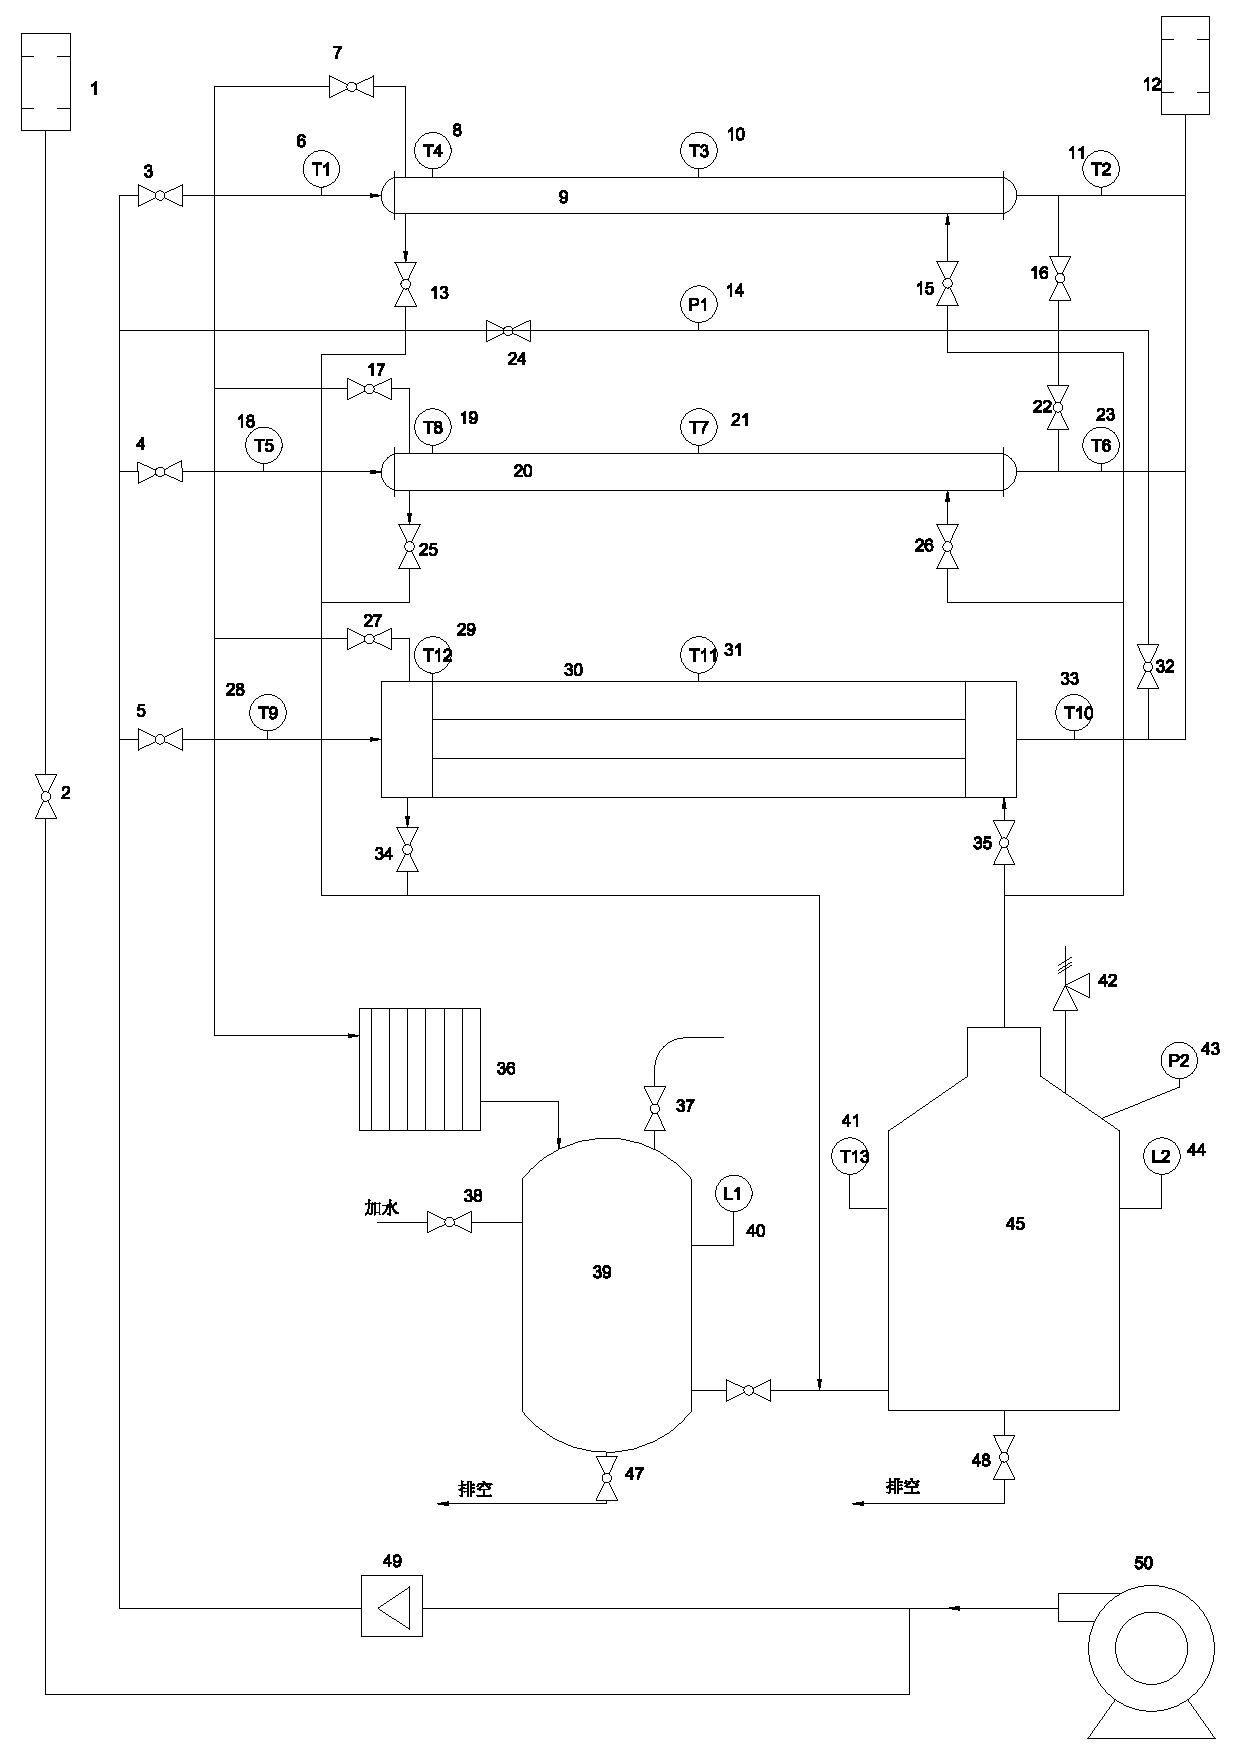
\includegraphics[width=0.7\linewidth]{Drawing1(cad2pdf).pdf}
    \caption{本实验的装置图}
    \label{fig:enter-label}
\end{figure}


    实验所使用的设备如下:
    \begin{itemize}
        \item HG1-5型风机(210$m^3/h$,200mbar)
        \item 功率为3Kw的蒸汽发生器
        \item 普通套管换热器
        \item 螺纹套管换热器
        \item 涡轮流量计, 温度传感器, 差压变送器
        \item 控制箱, 设备控制模块
    \end{itemize}


        \section{实验步骤}

        \begin{enumerate}
            \item 关闭所有阀门,启动总电源和仪表电源.
            \item 检查蒸汽发生器液位是否正常, 若不正常则补液,正常则设定加热温度, 启动蒸汽发生器.
            \item 全开冷空气支路调节阀, 全开a换热器的切换阀, 启动风机
            \item 蒸汽温度上升到100摄氏度时开启蒸汽进口阀,缓慢升温。稍微开启排空阀排除壳程中的不凝气体。开启冷凝液出口阀排出壳程中的冷凝液. 
            \item 稳定10~15分钟,当换热器壳层蒸汽温度达到100摄氏度时记录冷空气流量、冷空气进出口温度和蒸汽温度。
            \item 调节空气支路调节阀2,改变冷空气流量,稳定3分钟左右,记录冷空气流量、进出口温度和蒸汽温度。重复此操作,记录10组数据. 
            \item 重复3到6步操作完成b换热器的测定
            \item 关闭蒸汽发生器, 壳程温度降低到80摄氏度以下时关闭蒸汽进口阀, 排空阀和冷凝液出口阀, 以此关闭风机电源,仪表电源和总电源. 
        \end{enumerate}
\newpage
        \section{实验原始数据记录列表}

        \begin{figure}[h]
            \centering
            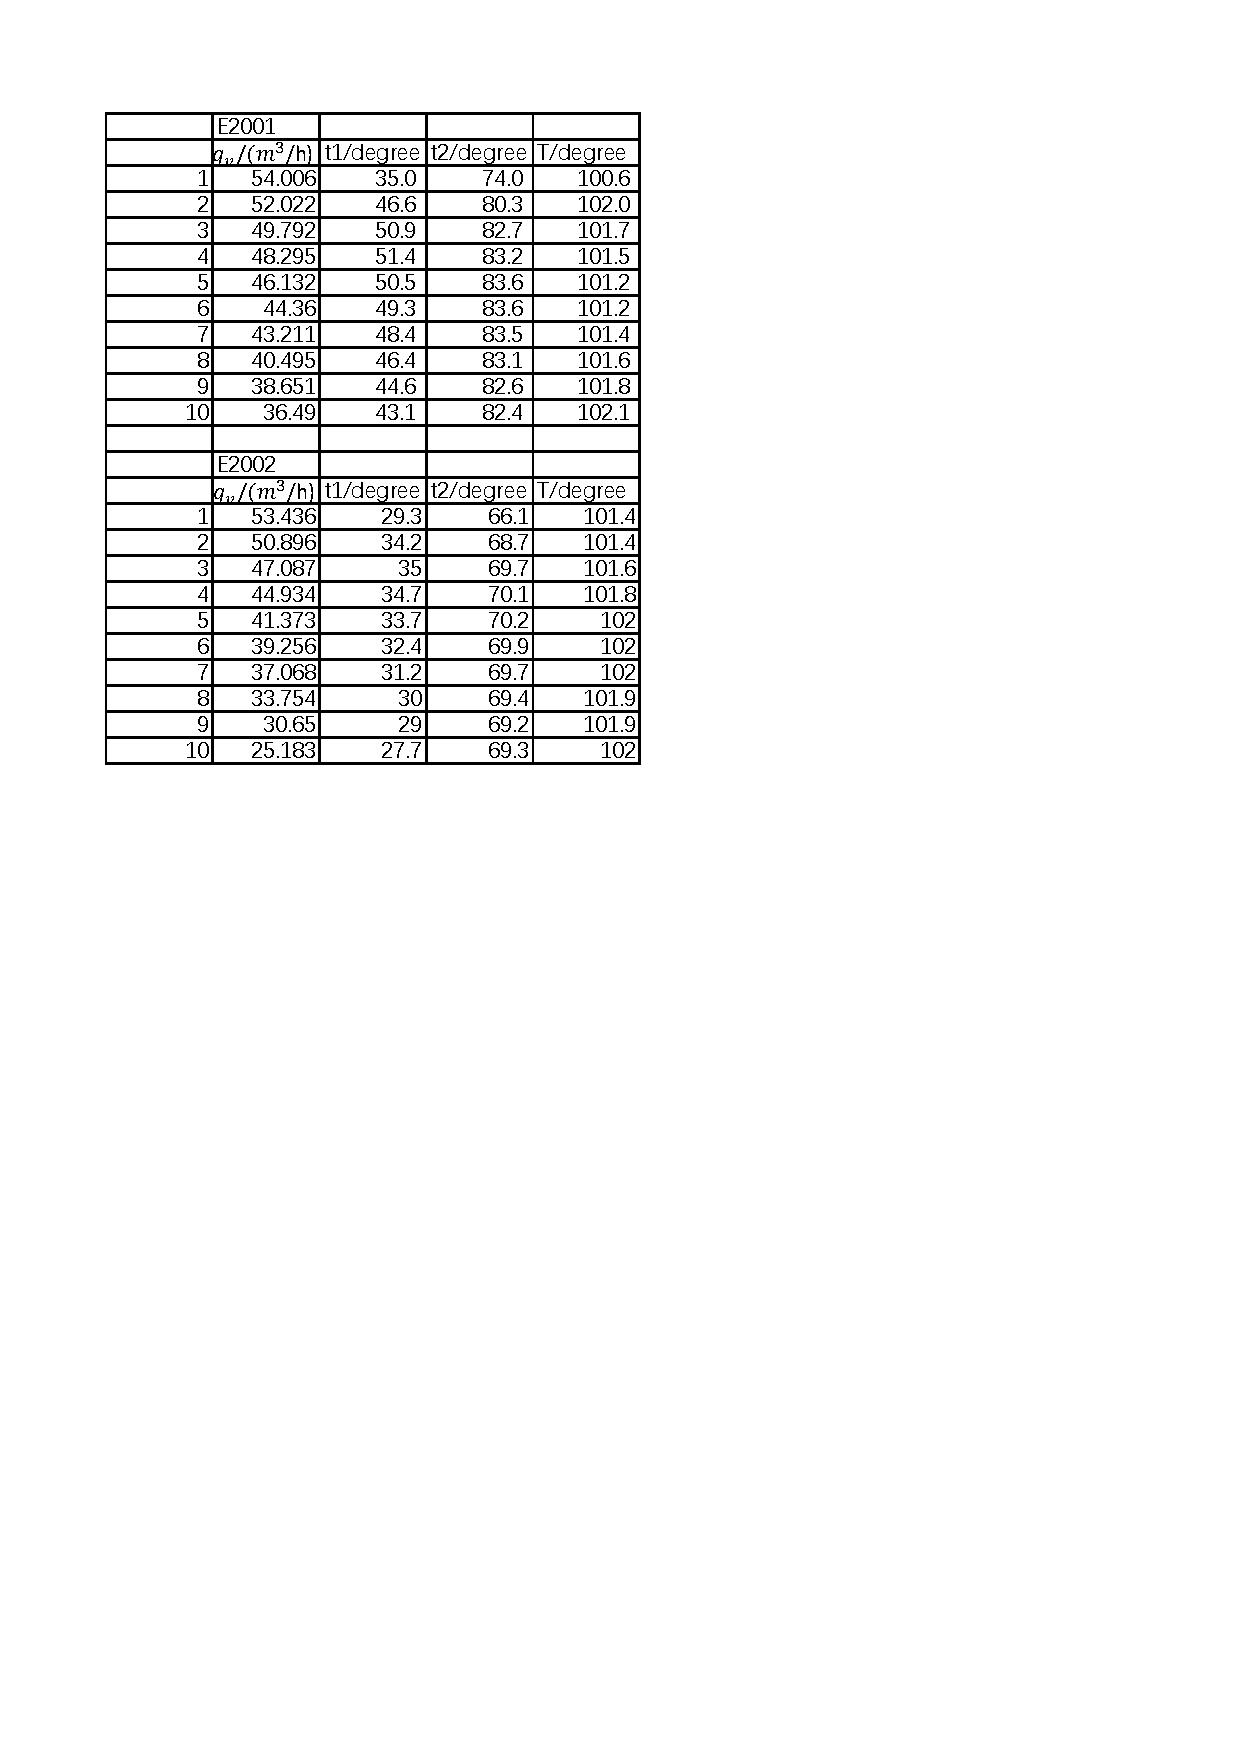
\includegraphics[width=0.7\linewidth]{7th_orig.pdf}
            \caption{本实验的原始数据}
            \label{fig:enter-label}
        \end{figure}
        
        \section{实验数据处理(以一组实验数据为例进行计算)}
        这里我们以E2001的第一组数据为例进行计算, 首先以进口温度和出口温度的平均为定性温度,查得在此温度下空气的密度为1,067$kg/m^3$, 粘度为$1.96*10^{-5}pa*s$, 比热容为$1009J/(Kg*K)$ ,热传导系数为$0.0285W/(M*k)$

        之后先算出进口处压差$\Delta t_1=65.6$摄氏度, 出口处压差$\Delta t_1=26.6$摄氏度, 然后计算对数平均温差:
$$\Delta T = \frac{\Delta t_1-\Delta t_{2}}{\ln\frac{\Delta t_1}{\Delta t_2}}=43.2^\circ C$$

因此传热功率为:
$$Q=q_v\rho C_p (t_2 -t_1)=629.89W$$

以内壁面为基准的总传热系数为:
$$K=\frac{Q}{k\pi d_i l}=193.39W/(m^2*K)$$

普朗特数为:
$$Pr=\frac{c_p \mu}{k}=0.694$$

努塞尔数为:
$$Nu=\frac{hd}{k}=135,71$$

雷诺数为:
$$\frac{\rho u d_i}{\mu}=52000$$

用同样的方法可以算出其余组的雷诺数,努塞尔数以及普朗特数.

        
        
        \section{实验结果(列表和作图)、结论与分析}
\subsection{实验结果}
        本实验的结果如下:
\begin{figure}[h]
    \centering
    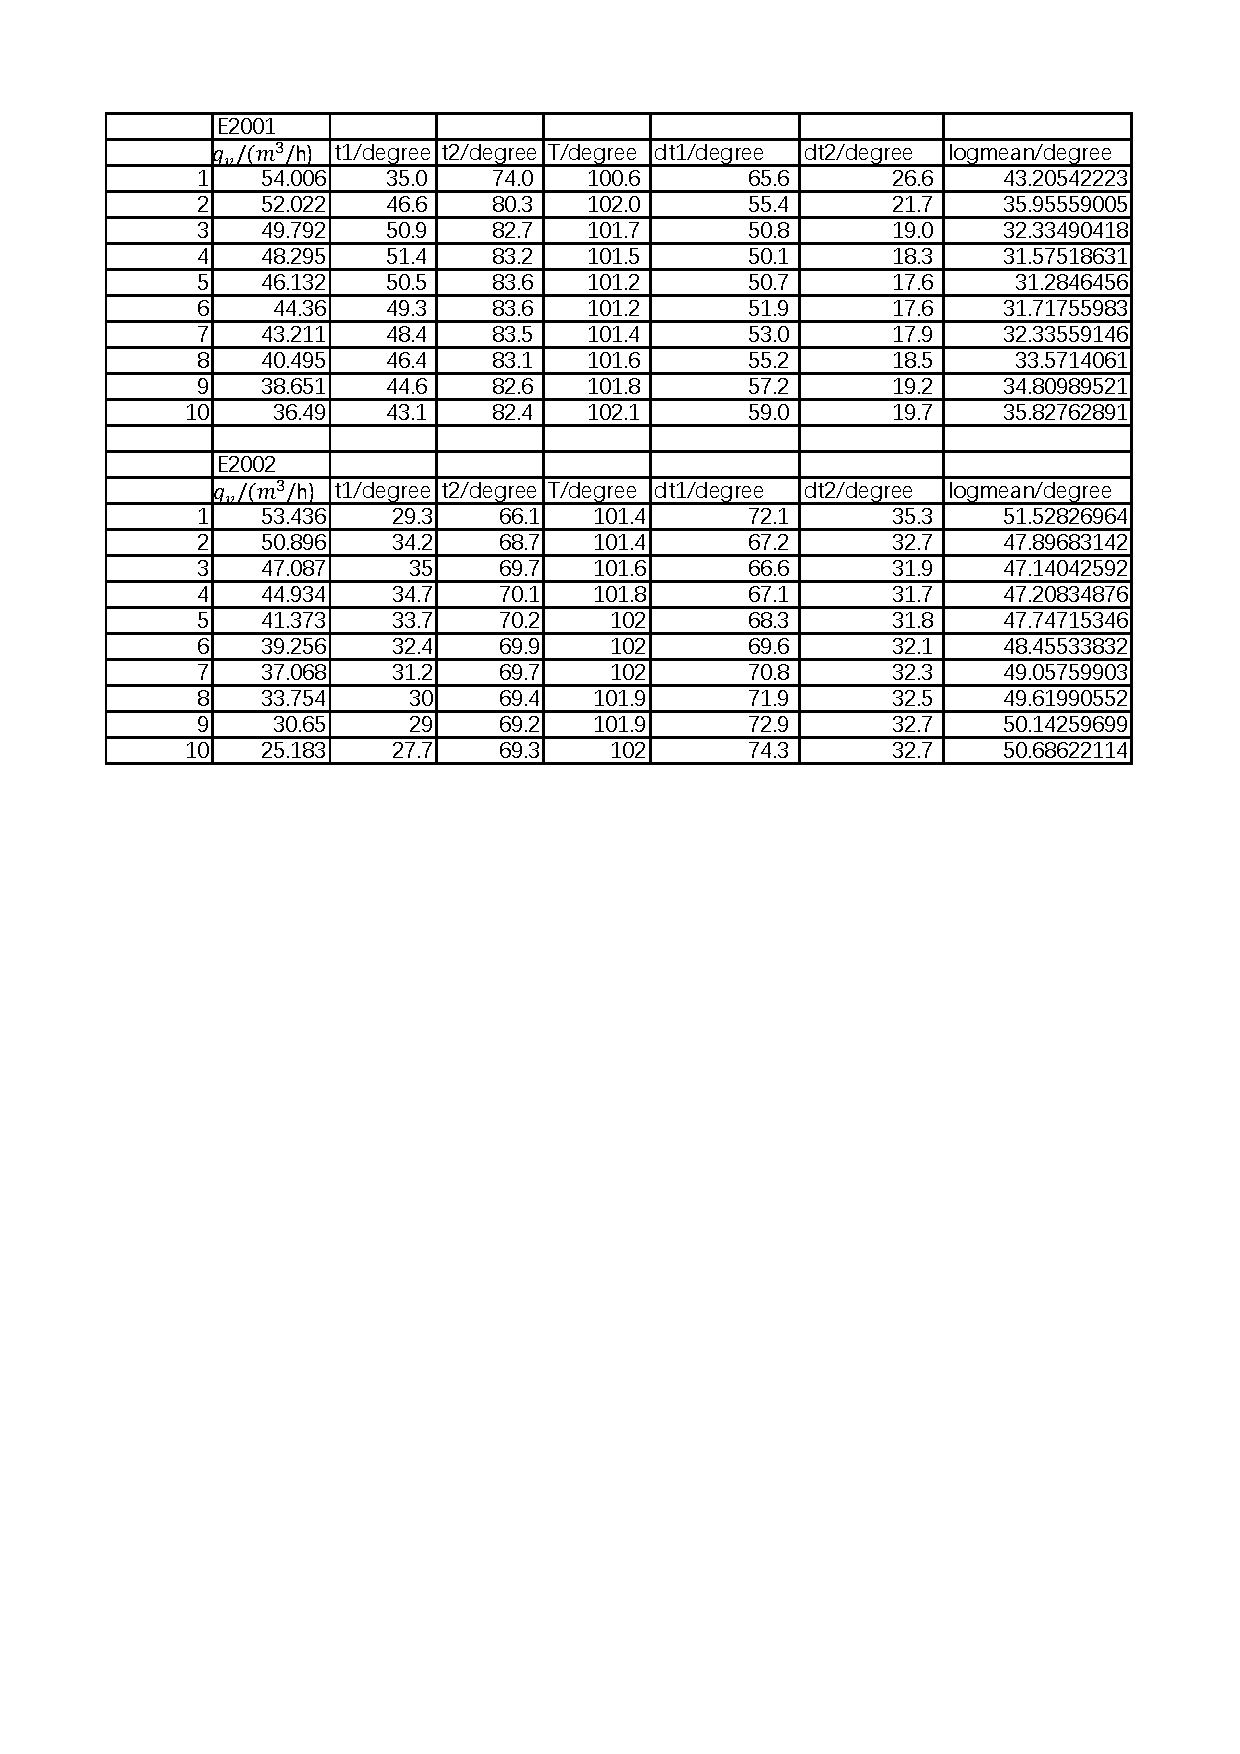
\includegraphics[width=0.7\linewidth]{7th.pdf}
    \caption{实验结果列表}
    \label{fig:enter-label}
\end{figure}
\newpage
根据计算结果做出的a换热器$\frac{Nu}{Pr^{0.4}}$随雷诺数变化曲线如下:
\begin{figure}[h]
    \centering
    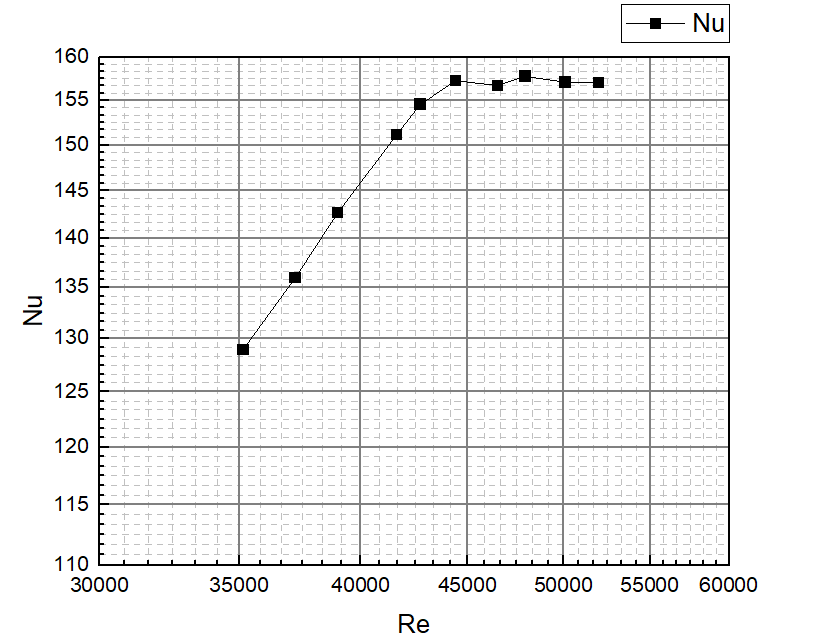
\includegraphics[width=0.6\linewidth]{image.png}
    \caption{a换热器$\frac{Nu}{Pr^{0.4}}$随雷诺数变化曲线}
    \label{fig:enter-label}
\end{figure}

b换热器$\frac{Nu}{Pr^{0.4}}$随雷诺数变化曲线如下:
\begin{figure}[h]
    \centering
    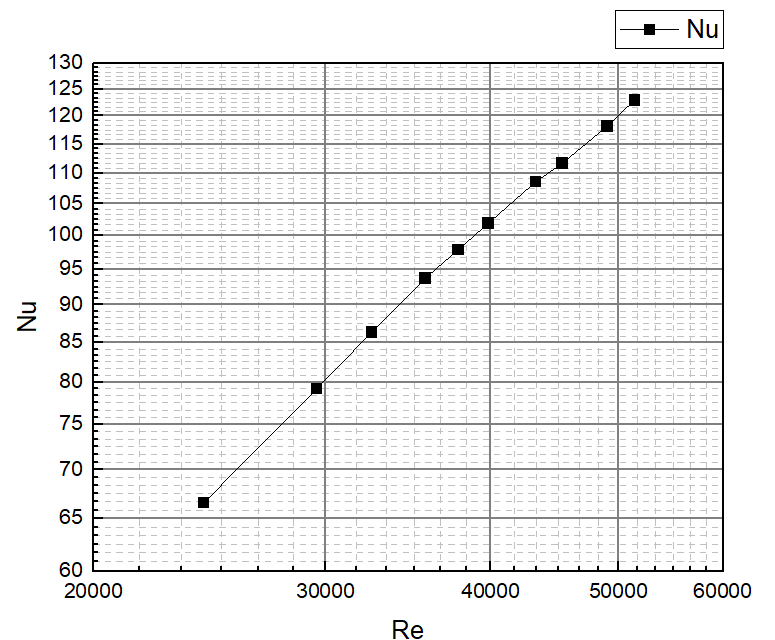
\includegraphics[width=0.6\linewidth]{imwdqage.png}
    \caption{b换热器$\frac{Nu}{Pr^{0.4}}$随雷诺数变化曲线}
    \label{fig:enter-label}
\end{figure}
\subsection{分析与结论}
a换热器的最后几组数据中${Nu}{Pr^{0.4}}$随雷诺数变化偏离了曲线,其原因可能是测这机组数据时没有等到稳态传热再测,而是调整阀门后直接测量了数据,从而导致很大的偏差. b换热器的实验结果符合预期,在双对数坐标系下$\frac{Nu}{Pr^{0.4}}$与雷诺数的关系符合一条直线. 在雷诺数相等时E2001的努塞尔数更大,所以初步推测E2001为内螺纹套管换热器. 

        \section{实验思考题}
	1. 分析影响传热系数及给热系数的因素。

    答:首先是流体的物性(如导热系数、密度、比热容和黏度)、流动状态(层流或湍流)以及流速,流速增加通常会增强对流传热;换热表面特性(如表面粗糙度和清洁程度)也会显著影响热阻,污垢或表面沉积物会降低给热系数;此外,换热设备的结构(如管径、管长和布置方式)以及冷热流体之间的温差和流动方式(并流、逆流或交叉流)也有一定影响。

    2.采取何种措施可提高K和h值?

    答: 可以通过增加流速, 定期清洁换热器, 使用内螺纹换热器, 选择合适的流动方式等措施来提高.

    3.tm、$\Delta tm$的物理意义是什么?如何确定?

    
    答:tm是定性温度,是进出口温度的算数平均,$\Delta tm$是对数平均温差,物理意义是传热推动力

    4.实验中管壁温度应接近哪一侧温度?为什么?

    答:更接近蒸汽测, 因为蒸汽侧的给热系数更大. 
	
	% 后记(附录)
	%%----------------------------------------------
%	附录Appendix
\appendix{
			\chapter{数据处理所涉及的代码或操作}
   \section{Python 代码}
\begin{lstlisting}[language= Python]
import numpy as np
import scipy as sp

\end{lstlisting}

\section{Origin 操作}
\begin{enumerate}
    \item 打开软件
\end{enumerate}
}
	
	
	% 参考文献
	%\addcontentsline{toc}{chapter}{参考文献}			% 在目录中添加参考文献
	%\bibliographystyle{unsrt}
	%\bibliography{ref/refs}
	
	% 声明
        \addcontentsline{toc}{chapter}{声\hspace{0.8cm}明}
	\section*{声\hspace{0.8cm}明}


%-------------------------------------------------------------------
	本人声明所呈交的实验报告是本人在教师指导下进行的实验工作及取得的实验成果。据我所知,除了文中特别加以标注和致谢的地方外,报告中不包含其他人已经发表或撰写过的成果,也不包含为获得四川大学或其他教育机构的学位或证书而使用过的材料。与我一同工作的同志对本实验所做的任何贡献均已在中作了明确的说明并表示谢意。
	
	本实验报告成果是本人在四川大学修读课程化工原理及仿真实验期间在教师指导下取得的,报告没有所有权归属。任何组织或个人被允许以任何合法目的,在不取得任何许可的情况下使用此报告中的部分或全部内容且需要承担由此引发的全部后果,特此声明。
	
	\vspace{40pt}
	\begin{flushright}
		\begin{tabular}{b{4cm} >{\centering\arraybackslash}b{2.5cm} }
			\songti \zihao{-4} 实验报告作者(签名)& {} \\[-3pt] 
			\cline{2-2} \\ [0.6cm]
                \songti \zihao{-4} 报告指导教师(签名)& {} \\[-3pt] 
			\cline{2-2} \\ [0.6cm]
		\end{tabular}
		
		\today
	\end{flushright}
	
	


	
	
\end{document} 
	